%%%%%%%%%%%%%%%%%%%%%%%%%%%%%%%%%%%%%%%%%%%%%%%%%%%%%%%%%%%%%%%%%%
% Sample template for MIT Junior Lab Student Written Summaries
% Available from http://web.mit.edu/8.13/www/Samplepaper/sample-paper.tex
%
% Last Updated August 30, 2011
%
% Adapted from the American Physical Societies REVTeK-4.1 Pages
% at http://publish.aps.org
%
% ADVICE TO STUDENTS: Each time you write a paper, start with this
% template and save under a new filename. If convenient, don't
%    erase unneeded lines, just comment them out.  Often, they
%    will be useful containers for information.
%
% Using pdflatex, images must be either PNG, GIF, JPEG or PDF.
%     Turn eps to pdf using epstopdf.
%%%%%%%%%%%%%%%%%%%%%%%%%%%%%%%%%%%%%%%%%%%%%%%%%%%%%%%%%%%%%%%%%%


%%%%%%%%%%%%%%%%%%%%%%%%%%%%%%%%%%%%%%%%%%%%%%%%%%%%%%%%%%%%%%%%%%
% PREAMBLE
% The preamble of a LaTeX document is the set of commands that precede
% the \begin{document} line.  It contains a \documentclass line
% to load the REVTeK-4.1 macro definitions and various \usepackage
% lines to load other macro packages.
%
% ADVICE TO STUDENTS: This preamble contains a suggested set of
% class options to generate a ``Junior Lab'' look and feel that
% facilitate quick review and feedback from one's peers, TA's
% and section instructors. Don't make substantial changes without
%     first consulting your section instructor.
%%%%%%%%%%%%%%%%%%%%%%%%%%%%%%%%%%%%%%%%%%%%%%%%%%%%%%%%%%%%%%%%%%

\documentclass[aps,twocolumn,secnumarabic,balancelastpage,amsmath,amssymb,nofootinbib]{revtex4}
%\documentclass[aps,twocolumn,secnumarabic,balancelastpage,amsmath,amssymb,nofootinbib]{revtex4-1}
\pdfpagewidth 8.5in
\pdfpageheight 11in

\usepackage{lgrind} % convert program listings to a form includable in a LaTeX document
\usepackage{chapterbib} % allows a bibliography for each chapter(each labguide has it's own)
\usepackage{color} % produces boxes or entire pages with coloredbackgrounds
\usepackage{graphics}      % standard graphics specifications
\usepackage[pdftex]{graphicx} % alternative graphics specifications
\usepackage{longtable}     % helps with long table options
\usepackage{epsf} % old package handles encapsulated post scriptissues
\usepackage{bm}            % special 'bold-math' package
%\usepackage{asymptote} % For typesetting of mathematical illustrations
\usepackage{thumbpdf}
\usepackage[colorlinks=true]{hyperref} % this package should be added after all others
% use as follows: \url{http://web.mit.edu/8.13}
\usepackage{multirow}
\usepackage{subfigure}

% Define a useful new command for writing units
\newcommand{\cd}{$\cdot$}

%
% And now, begin the document...
%

\begin{document}
\title{Nuclear Magnetic Resonance}
\author{Jay M.\ Lawhorn}
\email{klawhorn@mit.edu}
\date{\today}
\affiliation{MIT Department of Physics}

\begin{abstract}
Nuclear magnetic resonance exists!
\end{abstract}

\maketitle

Early work in nuclear magnetic resonance (NMR) was done by Isidor Rabi, Felix Bloch, and Edward Purcell.

The apparatus consists of a permament magnet that produces a static magnetic field and a probe circuit that delivers a radio frequency (RF) pulse and detects the resulting signal. 

The RF pulses are generated by a 15 MHz frequency synthesizer and fed through a power splitter which sends half of the signal to a double-balanced mixer and the other half to a phase detector for the output. The double-balanced mixer serves as a gate for the RF signal and is controlled by a micro-controller based digital pulse programmer which sets the pulse widths and timings. The RF signal is then amplifed and sent to the probe circuit. 

The sample under study is enclosed in a ten-turn copper coil which serves as an inductor in a tuned LC circuit.

The static magnetic field was measured with a Hall magnetometer as $1760\pm30$ G, including systematic uncertainties from the Hall magnetometer calibration and measurement.


%\begin{figure}[htb]
%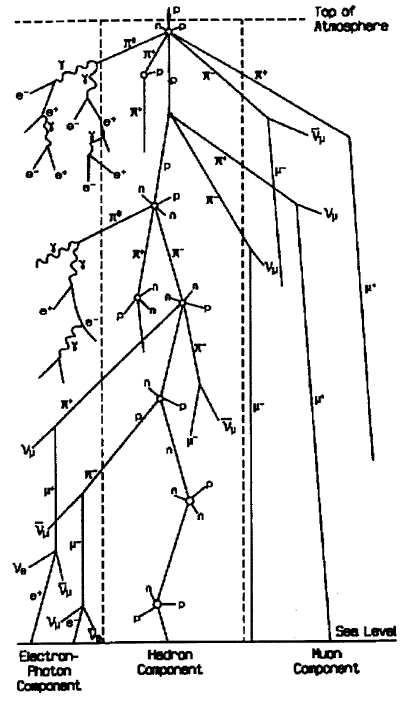
\includegraphics[width=7cm]{muon_shower.png}
%\caption{Figure showing the production of muons and other particles from cosmic rays. From\cite{grieder}.}
%\label{fig:muon_shower}
%\end{figure}

\end{document}
